\documentclass{article}

\usepackage[most]{tcolorbox}
\usepackage{physics}
\usepackage{graphicx}
\usepackage{float}
\usepackage{amsmath}
\usepackage{amssymb}


\usepackage[utf8]{inputenc}
\usepackage[a4paper, margin=1in]{geometry} % Controla los márgenes
\usepackage{titling}

\title{Clase 21 }
\author{Manuel Garcia.}
\date{\today}

\renewcommand{\maketitlehooka}{%
  \centering
  \vspace*{0.05cm} % Espacio vertical antes del título
}

\renewcommand{\maketitlehookd}{%
  \vspace*{2cm} % Espacio vertical después de la fecha
}

\newcommand{\caja}[3]{%
  \begin{tcolorbox}[colback=#1!5!white,colframe=#1!25!black,title=#2]
    #3
  \end{tcolorbox}%
}

\begin{document}
\maketitle

\section{}
Tenemos la funcion $ f(z) = \frac{1}{z } $, su integral de camino cerrado será: 
\begin{gather*}
  \displaystyle\oint_{P }^{} f(z) dz = 2\pi i 
\end{gather*}

\hfill 

\hfill 

\begin{gather*}
  \displaystyle\oint_{P }^{} f(z,z^*) dz = 2i \displaystyle\int_{S_P }^{} \frac{\partial f  }{\partial z^* }dxdy
\end{gather*}
Ya que $ \displaystyle\oint_{}^{} \frac{1}{z } dz = 2i \displaystyle\int_{S_P }^{} \frac{\partial  }{\partial z^* }\frac{1}{z }dz $ lo cual es igual a $ 0  $ o a $ 2\pi  $
\begin{gather*}
  \displaystyle\oint_{P }^{} f(z,z^*) dz = 2i \displaystyle\int_{S_P }^{} \frac{\partial f  }{\partial z^* }dxdy \\
  \frac{\partial  }{\partial z^* }\frac{1}{z } = \frac{1}{2} (\partial_x + i \partial _y ) \frac{1}{x + i y }  = \frac{1}{2}\left[\frac{-1 }{(x + i y )^2} + \frac{-i }{(x + i y )^2}\right]
\end{gather*}

\begin{gather*}
  \frac{\partial  }{\partial z^* } \frac{1}{z } = 0 \qquad z\neq 0 
\end{gather*}

Entonces: 
\begin{gather*}
  \frac{\partial  }{\partial z^* }\frac{1}{z } = \pi \delta(x) \delta(y) 
\end{gather*}

\hfill 

\hfill 

Si $ f(z) =z^*  $ 
\begin{gather*}
  \displaystyle\oint_{P }^{} z^* dz = 2i \underset{=A }{\displaystyle\int_{S_P }^{}dxdy }\\
  A = \frac{1}{2i }\displaystyle\oint_{P}^{} z^* dz 
\end{gather*}

\section{Caminos no simples y el número de winding }

\begin{gather*}
  \displaystyle\oint_{P }^{} \frac{dz }{z - z_0 } = \begin{cases}
    2\pi i \qquad &\text{si }z_0 \in S_P \\
    0 &\text{si }z_0 \notin S_P
  \end{cases}
\end{gather*}

\textbf{Ejemplo } 
\begin{gather*}
  \displaystyle\oint_{P}^{} \frac{z }{(z-i)(z-1)}dz 
\end{gather*}
Podemos dividir este camino no simple en dos caminos simples: 

\begin{figure}[H]
  \begin{center}
    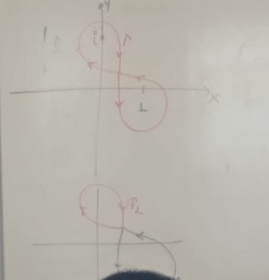
\includegraphics[width=0.3\textwidth]{camino_complejo.png}
  \end{center}
\end{figure}


\begin{gather*}
  \frac{z }{(z-i)(z-1)} = \frac{a}{z-i }\frac{b }{z-1 } \frac{a(z-1)+b(z-i ) }{(z-i)(z-1)}\\
  a = \frac{1-i }{2 }\qquad b = \frac{1 +i }{2 } \\
  \frac{z }{(z-i)(z-1)} = \frac{1}{2}\left[\frac{1 - i }{z-i } + \frac{1 + i }{z - 1 }\right] 
\end{gather*}

La integral nos queda: 
\begin{gather*}
  \displaystyle\oint_{P }^{} f(z)dz = \frac{1}{2}\left[\displaystyle\oint_{P_1 }^{} \frac{1 - i }{z - i } dz + \displaystyle\oint_{P_1 }^{} \frac{1 + i }{z - 1 }dz + \displaystyle\oint_{P_2 }^{} \frac{1 - i }{z - i } dz + \displaystyle\oint_{P_2 }^{} \frac{1 + i }{z - 1 }dz\right]
\end{gather*}
Calculando las integrales: $ \oint_{P_1} \frac{1}{z-i }dz = -2 \pi i  \qquad \oint_{P_2} \frac{1}{z - 1 } dz = 2 \pi i  $, recordemos que se tuvo en cuenta la direccion del camino para los signos.

\begin{gather*}
  \displaystyle\oint_{P }^{} f(z)dz = \frac{1}{2}(1 - i )(-2\pi i ) + \frac{1}{2}(1 + i )(2\pi i ) = - 2 \pi  
\end{gather*}

\subsection{Numero de Winding}

\begin{figure}[H]
  \begin{center}
    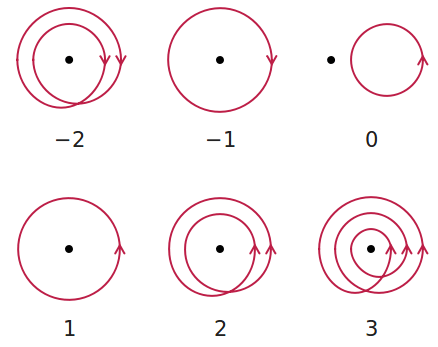
\includegraphics[width=0.4\textwidth]{numeros_winding.png}
  \end{center}
\end{figure}

El número de Winding (zigzageante o sepenteante) $ \gamma $ asociado a un camino $ \Gamma  $ cerrado y al rededor del punto $ z_0  $, que denotaremos $ \gamma[P,z_0 ] $, es el número de rotaciones netas en sentido contrario a las manecillas del reloj que el camino P rodea el punto $ z_0  $.
\begin{figure}[H]
  \begin{center}
    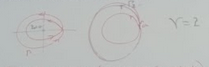
\includegraphics[width=0.5\textwidth]{numero_winding.png}
  \end{center}
\end{figure}
\begin{gather*}
  \displaystyle\oint_{P }^{} \frac{1}{z - z_0 }dz = 2\pi i \gamma[P,z_0 ] = 2\pi i 2 = 4\pi i 
\end{gather*}

\textbf{Ejemplo } $ \displaystyle\oint_{P }^{} z ^* dz  $ 
\begin{figure}[H]
  \begin{center}
    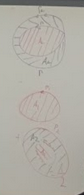
\includegraphics[width=0.3\textwidth]{ej2.png}
  \end{center}
\end{figure}
\begin{align*}
  \displaystyle\oint_{P }^{} z ^* dz &= \displaystyle\oint_{P_1 }^{} z ^* dz+ \displaystyle\oint_{P_2 }^{} z ^* dz\\
        &= 2 i A_1 + 2 i (A_1 + A_2)\\
        &= 2i \left[2A_1 + A_2 \right] \\
        &= 2i \left[A_1 \gamma(P,z_1) + A_2 \gamma(P,z_2 )\right]
\end{align*}
Tenemos que: 
\caja{red}{}{
  \begin{align*}
    \displaystyle\oint_{P }^{}z^*dz  &= \displaystyle\sum_{j }^{}A_j \gamma[P,z_j ], \qquad z_j \in A_j \\
      &= \displaystyle\sum_{j }^{}\gamma_j A_j 
  \end{align*}
  $ A  $ es el area geometrica.
}

\caja{green}{Formula integral de Cauchy }{
  Si $ F(z)  $ es analitica dentro del dominio $ \Gamma  $ encerrado por $ \beta $ y en $ \beta $, entonces: 
  \begin{gather*}
    f(a) = \frac{1}{2\pi i } \displaystyle\oint_{\beta }^{} \frac{f(z) dz }{z-a } 
  \end{gather*}
}

\caja{green}{Teorema de acotacion }{
  $ \beta, f(z)  $ sobre $ P  $ está acotada $ \left|F(z)\right| \leq M , \quad z \in \beta $
  \begin{align*}
    \oint_\beta f(z) dz &\leq \oint_\beta \left|f(z) \right|dz \qquad \oint_\beta f(z)dz \leq Ml(\beta) \\
    &\leq M \oint_\beta dz \\
    &= M l(\beta)
  \end{align*}
}


\end{document}
